\documentclass[12pt,]{book}
\usepackage{lmodern}
\usepackage{amssymb,amsmath}
\usepackage{ifxetex,ifluatex}
\usepackage{fixltx2e} % provides \textsubscript
\ifnum 0\ifxetex 1\fi\ifluatex 1\fi=0 % if pdftex
  \usepackage[T1]{fontenc}
  \usepackage[utf8]{inputenc}
\else % if luatex or xelatex
  \ifxetex
    \usepackage{mathspec}
  \else
    \usepackage{fontspec}
  \fi
  \defaultfontfeatures{Ligatures=TeX,Scale=MatchLowercase}
\fi
% use upquote if available, for straight quotes in verbatim environments
\IfFileExists{upquote.sty}{\usepackage{upquote}}{}
% use microtype if available
\IfFileExists{microtype.sty}{%
\usepackage{microtype}
\UseMicrotypeSet[protrusion]{basicmath} % disable protrusion for tt fonts
}{}
\usepackage[left=4cm, right=3cm, top=2.5cm, bottom=2.5cm]{geometry}
\usepackage{hyperref}
\hypersetup{unicode=true,
            pdftitle={Psychophysiological characteristics of verbal rumination},
            pdfauthor={Ladislas Nalborczyk},
            pdfborder={0 0 0},
            breaklinks=true}
\urlstyle{same}  % don't use monospace font for urls
\usepackage{natbib}
\bibliographystyle{apalike}
\usepackage{color}
\usepackage{fancyvrb}
\newcommand{\VerbBar}{|}
\newcommand{\VERB}{\Verb[commandchars=\\\{\}]}
\DefineVerbatimEnvironment{Highlighting}{Verbatim}{commandchars=\\\{\}}
% Add ',fontsize=\small' for more characters per line
\usepackage{framed}
\definecolor{shadecolor}{RGB}{248,248,248}
\newenvironment{Shaded}{\begin{snugshade}}{\end{snugshade}}
\newcommand{\KeywordTok}[1]{\textcolor[rgb]{0.13,0.29,0.53}{\textbf{#1}}}
\newcommand{\DataTypeTok}[1]{\textcolor[rgb]{0.13,0.29,0.53}{#1}}
\newcommand{\DecValTok}[1]{\textcolor[rgb]{0.00,0.00,0.81}{#1}}
\newcommand{\BaseNTok}[1]{\textcolor[rgb]{0.00,0.00,0.81}{#1}}
\newcommand{\FloatTok}[1]{\textcolor[rgb]{0.00,0.00,0.81}{#1}}
\newcommand{\ConstantTok}[1]{\textcolor[rgb]{0.00,0.00,0.00}{#1}}
\newcommand{\CharTok}[1]{\textcolor[rgb]{0.31,0.60,0.02}{#1}}
\newcommand{\SpecialCharTok}[1]{\textcolor[rgb]{0.00,0.00,0.00}{#1}}
\newcommand{\StringTok}[1]{\textcolor[rgb]{0.31,0.60,0.02}{#1}}
\newcommand{\VerbatimStringTok}[1]{\textcolor[rgb]{0.31,0.60,0.02}{#1}}
\newcommand{\SpecialStringTok}[1]{\textcolor[rgb]{0.31,0.60,0.02}{#1}}
\newcommand{\ImportTok}[1]{#1}
\newcommand{\CommentTok}[1]{\textcolor[rgb]{0.56,0.35,0.01}{\textit{#1}}}
\newcommand{\DocumentationTok}[1]{\textcolor[rgb]{0.56,0.35,0.01}{\textbf{\textit{#1}}}}
\newcommand{\AnnotationTok}[1]{\textcolor[rgb]{0.56,0.35,0.01}{\textbf{\textit{#1}}}}
\newcommand{\CommentVarTok}[1]{\textcolor[rgb]{0.56,0.35,0.01}{\textbf{\textit{#1}}}}
\newcommand{\OtherTok}[1]{\textcolor[rgb]{0.56,0.35,0.01}{#1}}
\newcommand{\FunctionTok}[1]{\textcolor[rgb]{0.00,0.00,0.00}{#1}}
\newcommand{\VariableTok}[1]{\textcolor[rgb]{0.00,0.00,0.00}{#1}}
\newcommand{\ControlFlowTok}[1]{\textcolor[rgb]{0.13,0.29,0.53}{\textbf{#1}}}
\newcommand{\OperatorTok}[1]{\textcolor[rgb]{0.81,0.36,0.00}{\textbf{#1}}}
\newcommand{\BuiltInTok}[1]{#1}
\newcommand{\ExtensionTok}[1]{#1}
\newcommand{\PreprocessorTok}[1]{\textcolor[rgb]{0.56,0.35,0.01}{\textit{#1}}}
\newcommand{\AttributeTok}[1]{\textcolor[rgb]{0.77,0.63,0.00}{#1}}
\newcommand{\RegionMarkerTok}[1]{#1}
\newcommand{\InformationTok}[1]{\textcolor[rgb]{0.56,0.35,0.01}{\textbf{\textit{#1}}}}
\newcommand{\WarningTok}[1]{\textcolor[rgb]{0.56,0.35,0.01}{\textbf{\textit{#1}}}}
\newcommand{\AlertTok}[1]{\textcolor[rgb]{0.94,0.16,0.16}{#1}}
\newcommand{\ErrorTok}[1]{\textcolor[rgb]{0.64,0.00,0.00}{\textbf{#1}}}
\newcommand{\NormalTok}[1]{#1}
\usepackage{longtable,booktabs}
\usepackage{graphicx,grffile}
\makeatletter
\def\maxwidth{\ifdim\Gin@nat@width>\linewidth\linewidth\else\Gin@nat@width\fi}
\def\maxheight{\ifdim\Gin@nat@height>\textheight\textheight\else\Gin@nat@height\fi}
\makeatother
% Scale images if necessary, so that they will not overflow the page
% margins by default, and it is still possible to overwrite the defaults
% using explicit options in \includegraphics[width, height, ...]{}
\setkeys{Gin}{width=\maxwidth,height=\maxheight,keepaspectratio}
\IfFileExists{parskip.sty}{%
\usepackage{parskip}
}{% else
\setlength{\parindent}{0pt}
\setlength{\parskip}{6pt plus 2pt minus 1pt}
}
\setlength{\emergencystretch}{3em}  % prevent overfull lines
\providecommand{\tightlist}{%
  \setlength{\itemsep}{0pt}\setlength{\parskip}{0pt}}
\setcounter{secnumdepth}{5}
% Redefines (sub)paragraphs to behave more like sections
\ifx\paragraph\undefined\else
\let\oldparagraph\paragraph
\renewcommand{\paragraph}[1]{\oldparagraph{#1}\mbox{}}
\fi
\ifx\subparagraph\undefined\else
\let\oldsubparagraph\subparagraph
\renewcommand{\subparagraph}[1]{\oldsubparagraph{#1}\mbox{}}
\fi

%%% Use protect on footnotes to avoid problems with footnotes in titles
\let\rmarkdownfootnote\footnote%
\def\footnote{\protect\rmarkdownfootnote}

%%% Change title format to be more compact
\usepackage{titling}

% Create subtitle command for use in maketitle
\newcommand{\subtitle}[1]{
  \posttitle{
    \begin{center}\large#1\end{center}
    }
}

\setlength{\droptitle}{-2em}

  \title{Psychophysiological characteristics of verbal rumination}
    \pretitle{\vspace{\droptitle}\centering\huge}
  \posttitle{\par}
    \author{Ladislas Nalborczyk}
    \preauthor{\centering\large\emph}
  \postauthor{\par}
      \predate{\centering\large\emph}
  \postdate{\par}
    \date{2018-09-04}

\usepackage{tikz}
\usepackage{lscape}
\usepackage{indentfirst}
\usepackage{float}
\usepackage[flushleft]{threeparttable}
\usepackage[fulladjust]{marginnote}
\usepackage{tcolorbox}
\usepackage{pdfpages}
\usetikzlibrary{intersections}
\tcbuselibrary{listings,breakable}
\usepackage{pifont}
\usepackage{hyperref}
\usepackage[utf8]{inputenc}
\usepackage{graphicx,pdflscape}
\usepackage{geometry}
\usepackage{float}
\usepackage{longtable}
\usepackage{supertabular}
\usepackage[flushleft]{threeparttable}
\usepackage{subfig}
\usepackage{scrextend}
\usepackage{tabularx}
\usepackage{lscape}
\usepackage{tabu}
\usepackage{array}
\usepackage[gen]{eurosym}
\usepackage{subfig}
\usepackage{stackrel,amssymb}
\usepackage{textcomp}
\usepackage{setspace}

\usepackage{booktabs,caption,fixltx2e}
\usepackage[none]{hyphenat}

%%%%%%%%%%%%%%%%%%%%%%%%%%%%%%%%%%%%%%%%%%%%%%%%%%%%%%%%%%%%%%%%%%%%%%%%%%%%%%%%%%%%%%%%%%
% below is the by-default configuration of bookdown-demo
% https://github.com/rstudio/bookdown-demo/blob/master/preamble.tex
%%%%%%%%%%%%%%%%%%%%%%%%%%%%%%%%%%%%%%%%%%%%%%%%%%%%%%%%%%%%%%%%%%%%%%%%%%%%%%%%

\usepackage{graphicx}
\usepackage{amsthm}

\makeatletter
\def\thm@space@setup{%
  \thm@preskip=8pt plus 2pt minus 4pt
  \thm@postskip=\thm@preskip
}
\makeatother

\begin{document}
\maketitle

{
\setcounter{tocdepth}{1}
\tableofcontents
}
\listoftables
\listoffigures
\chapter*{Welcome}\label{welcome}
\addcontentsline{toc}{chapter}{Welcome}

This book, when finished, will contain my dissertation research.

\chapter*{Acknowledgments}\label{acknowledgments}
\addcontentsline{toc}{chapter}{Acknowledgments}

Acknowledgemnents are not yet available.

\chapter*{Abstract}\label{abstract}
\addcontentsline{toc}{chapter}{Abstract}

Blah blah blah

\part{Theoretical
framework}\label{part-theoretical-framework}

\chapter{Overt and imagined actions}\label{intro}

\ldots{}

\section{Motor imagery}\label{motor-imagery}

Considerable experimental evidence has accumulated to suggest that
movement execution and MI share substantial overlap of active brain
regions (for review, see Guillot et al., 2012). Such apparent functional
equivalence supports the hypothesis that MI draws on the similar neural
networks that are used in actual perception and motor control
(Jeannerod, 1994; Grezes and Decety, 2001; Holmes and Collins,
2001)\ldots{}

\subsection{Simulation theories}\label{simulation-theories}

\ldots{}

\subsection{Emulation theories}\label{emulation-theories}

\ldots{}

\subsection{Action representation and internal
models}\label{action-representation-and-internal-models}

Voir Jeannerod (2004), Wolpert el al. (1995), Wolpert \& Gharamani
(2000)\ldots{}

\section{Speech imagery}\label{speech-imagery}

\ldots{}

\subsection{MVTV Cohen (1986)}\label{mvtv-cohen-1986}

\ldots{}

\subsection{Predictive models}\label{predictive-models}

\ldots{}

\chapter{Rumination as simulated
speech}\label{rumination-as-simulated-speech}

As suggested by \citet{Christoff2016}, rumination and other forms of
spontaneous thoughts can be considered in a common conceptual space (see
Figure 1). This space is built upon two dimensions: \emph{deliberate
constraints} and \emph{automatic constraints}. These dimensions
represent two general mechanisms that allow to constrain the contents of
these related mental states and the transitions between them. The first
contrain correspond to a deliberate processus and is implemented through
\textbf{cognitive control} \citep{Miller2000}. The second constrain is
referring to more automatic constrains like sensory afferences. In this
framework, rumination is characterized by the highest level of automatic
constraints and spread all along the \emph{deliberate constraints}
dimension.

\begin{figure}

{\centering 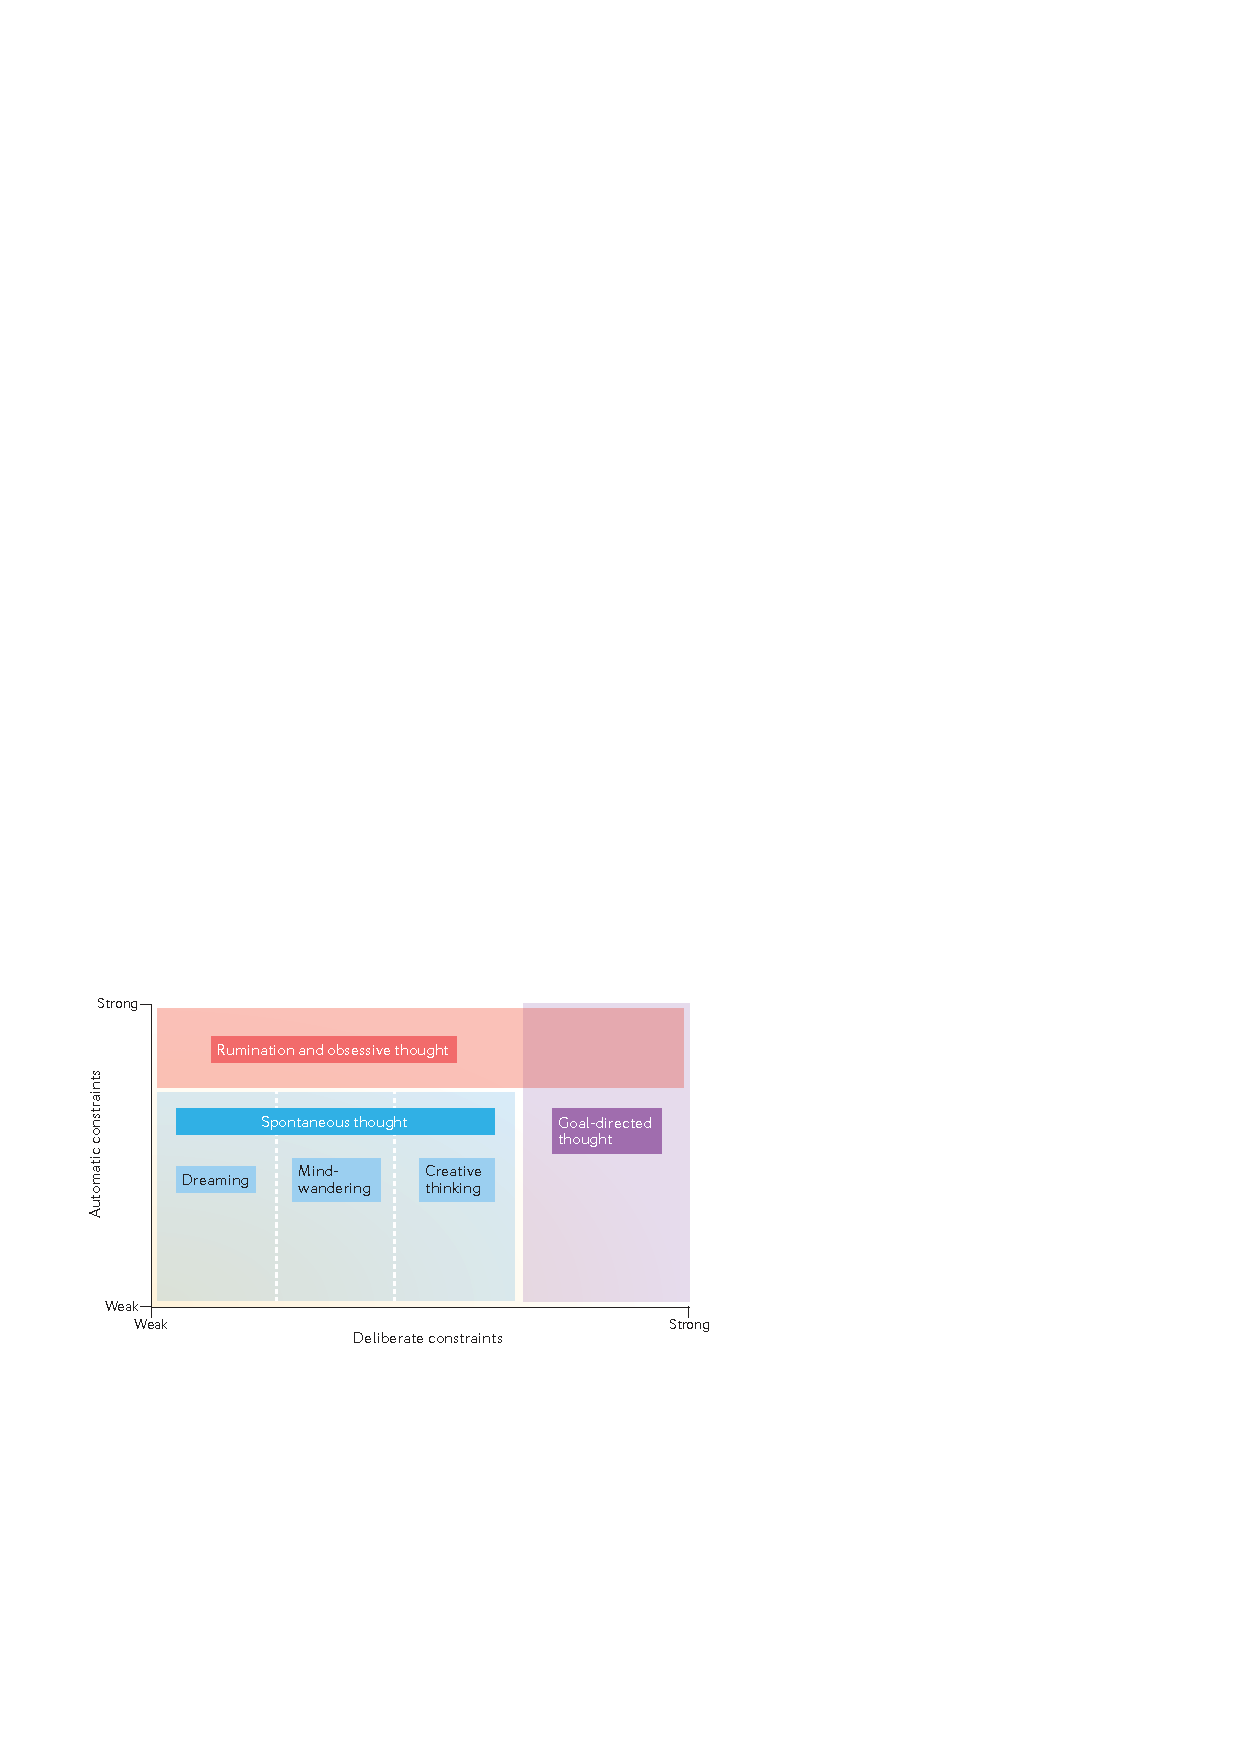
\includegraphics{assets/conceptual_space} 

}

\caption{Conceptual space of different types of thought (Christoff et al., 2016)}\label{fig:unnamed-chunk-1}
\end{figure}

\ldots{}

\chapter{Electromyographic correlates of speech
production}\label{electromyographic-correlates-of-speech-production}

\ldots{}

\section{Speech production
mechanisms}\label{speech-production-mechanisms}

\ldots{}

\section{Speech production muscles}\label{speech-production-muscles}

\ldots{}

\section{Muscular physiology}\label{muscular-physiology}

\ldots{}

\section{EMG signal}\label{emg-signal}

\subsection{EMG signal measures}\label{emg-signal-measures}

Muscular activity can be studied at different levels. At the cellular
level, using electrophysiological measures like micro-electrods
implanted in the cell, that allow direct measures of \textbf{action
potential}. At the segmental level, biomechanis study muscular activity
using surface sensors, positionned on the skin\ldots{}intermediate
levels\ldots{}

\subsection{Motor Unit Action
Potential}\label{motor-unit-action-potential}

\textbf{Motor unit action potential} (MUAP) is the electric field
resulting from the sum f the electric fiels emitted y each fiber of the
motor unit. This train of action potentials will generate a \emph{train}
of MUAP, call \textbf{motor unit action potential trains} (MUAPT). The
electric potential generated by this field is highly dependant of
parameters such as the number of fibers, their length, speed of
conduction and position of the neuromuscular junction.

\begin{figure}

{\centering 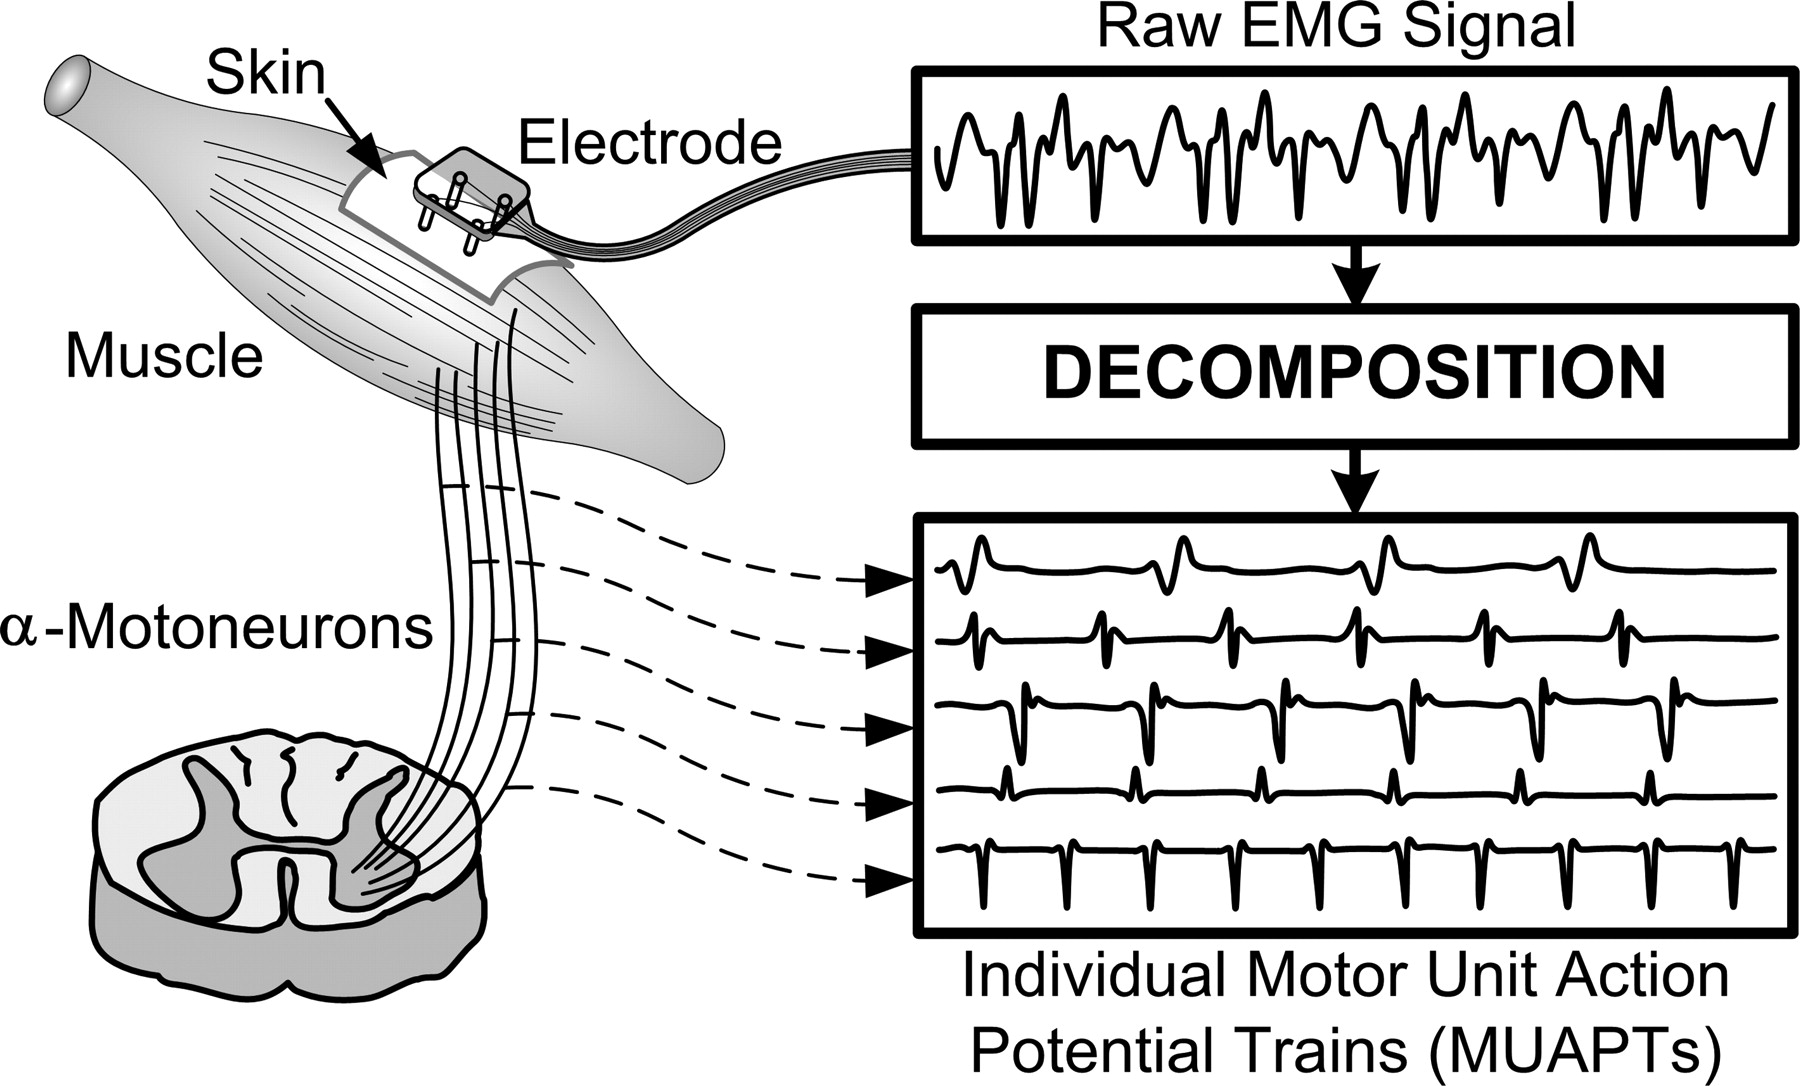
\includegraphics{assets/muap} 

}

\caption{Motor unit action potential schema.}\label{fig:unnamed-chunk-1}
\end{figure}

\ldots{}

EMG signal then result in a mixture of recruited motor units.

\subsection{Surface EMG}\label{surface-emg}

\ldots{}\emph{crosstalk} phenomenon \citep{DeLuca1997}. In reason of the
important\ldots{} of facial muscles, the EMG activity of one recorded
muscle generally does not represent the activity of a single muscle but
rather a mixture of\ldots{}\citet{Rapin2011}\ldots{}

\subsection{Basic signal processing}\label{basic-signal-processing}

\ldots{}the EMG signal is a stochastic signal\ldots{} In order to
illustrate what EMG signal looks like, we simulated EMG signal based on
a standard algorithm \citep[pp.70-71]{Hermens1999}, implemented in R by
\citet{Borg2014}.

\begin{Shaded}
\begin{Highlighting}[]
\OperatorTok{>}\StringTok{ }\KeywordTok{source}\NormalTok{(}\StringTok{"code/EMGfuns.R"}\NormalTok{)}
\OperatorTok{>}\StringTok{ }\NormalTok{emg <-}\StringTok{ }\KeywordTok{EMG_sim}\NormalTok{(}\DataTypeTok{n =} \DecValTok{2048}\NormalTok{, }\DataTypeTok{sampFreq =} \DecValTok{1000}\NormalTok{, }\DataTypeTok{lF =} \DecValTok{10}\NormalTok{, }\DataTypeTok{hF =} \DecValTok{100}\NormalTok{)}\OperatorTok{$}\NormalTok{sim}
\OperatorTok{>}\StringTok{ }\KeywordTok{ts.plot}\NormalTok{(emg, }\DataTypeTok{xlab =} \StringTok{"Time (ms)"}\NormalTok{, }\DataTypeTok{ylab =} \StringTok{"simEMG"}\NormalTok{, }\DataTypeTok{col =} \StringTok{"steelblue"}\NormalTok{)}
\end{Highlighting}
\end{Shaded}

\begin{figure}[h!]

{\centering 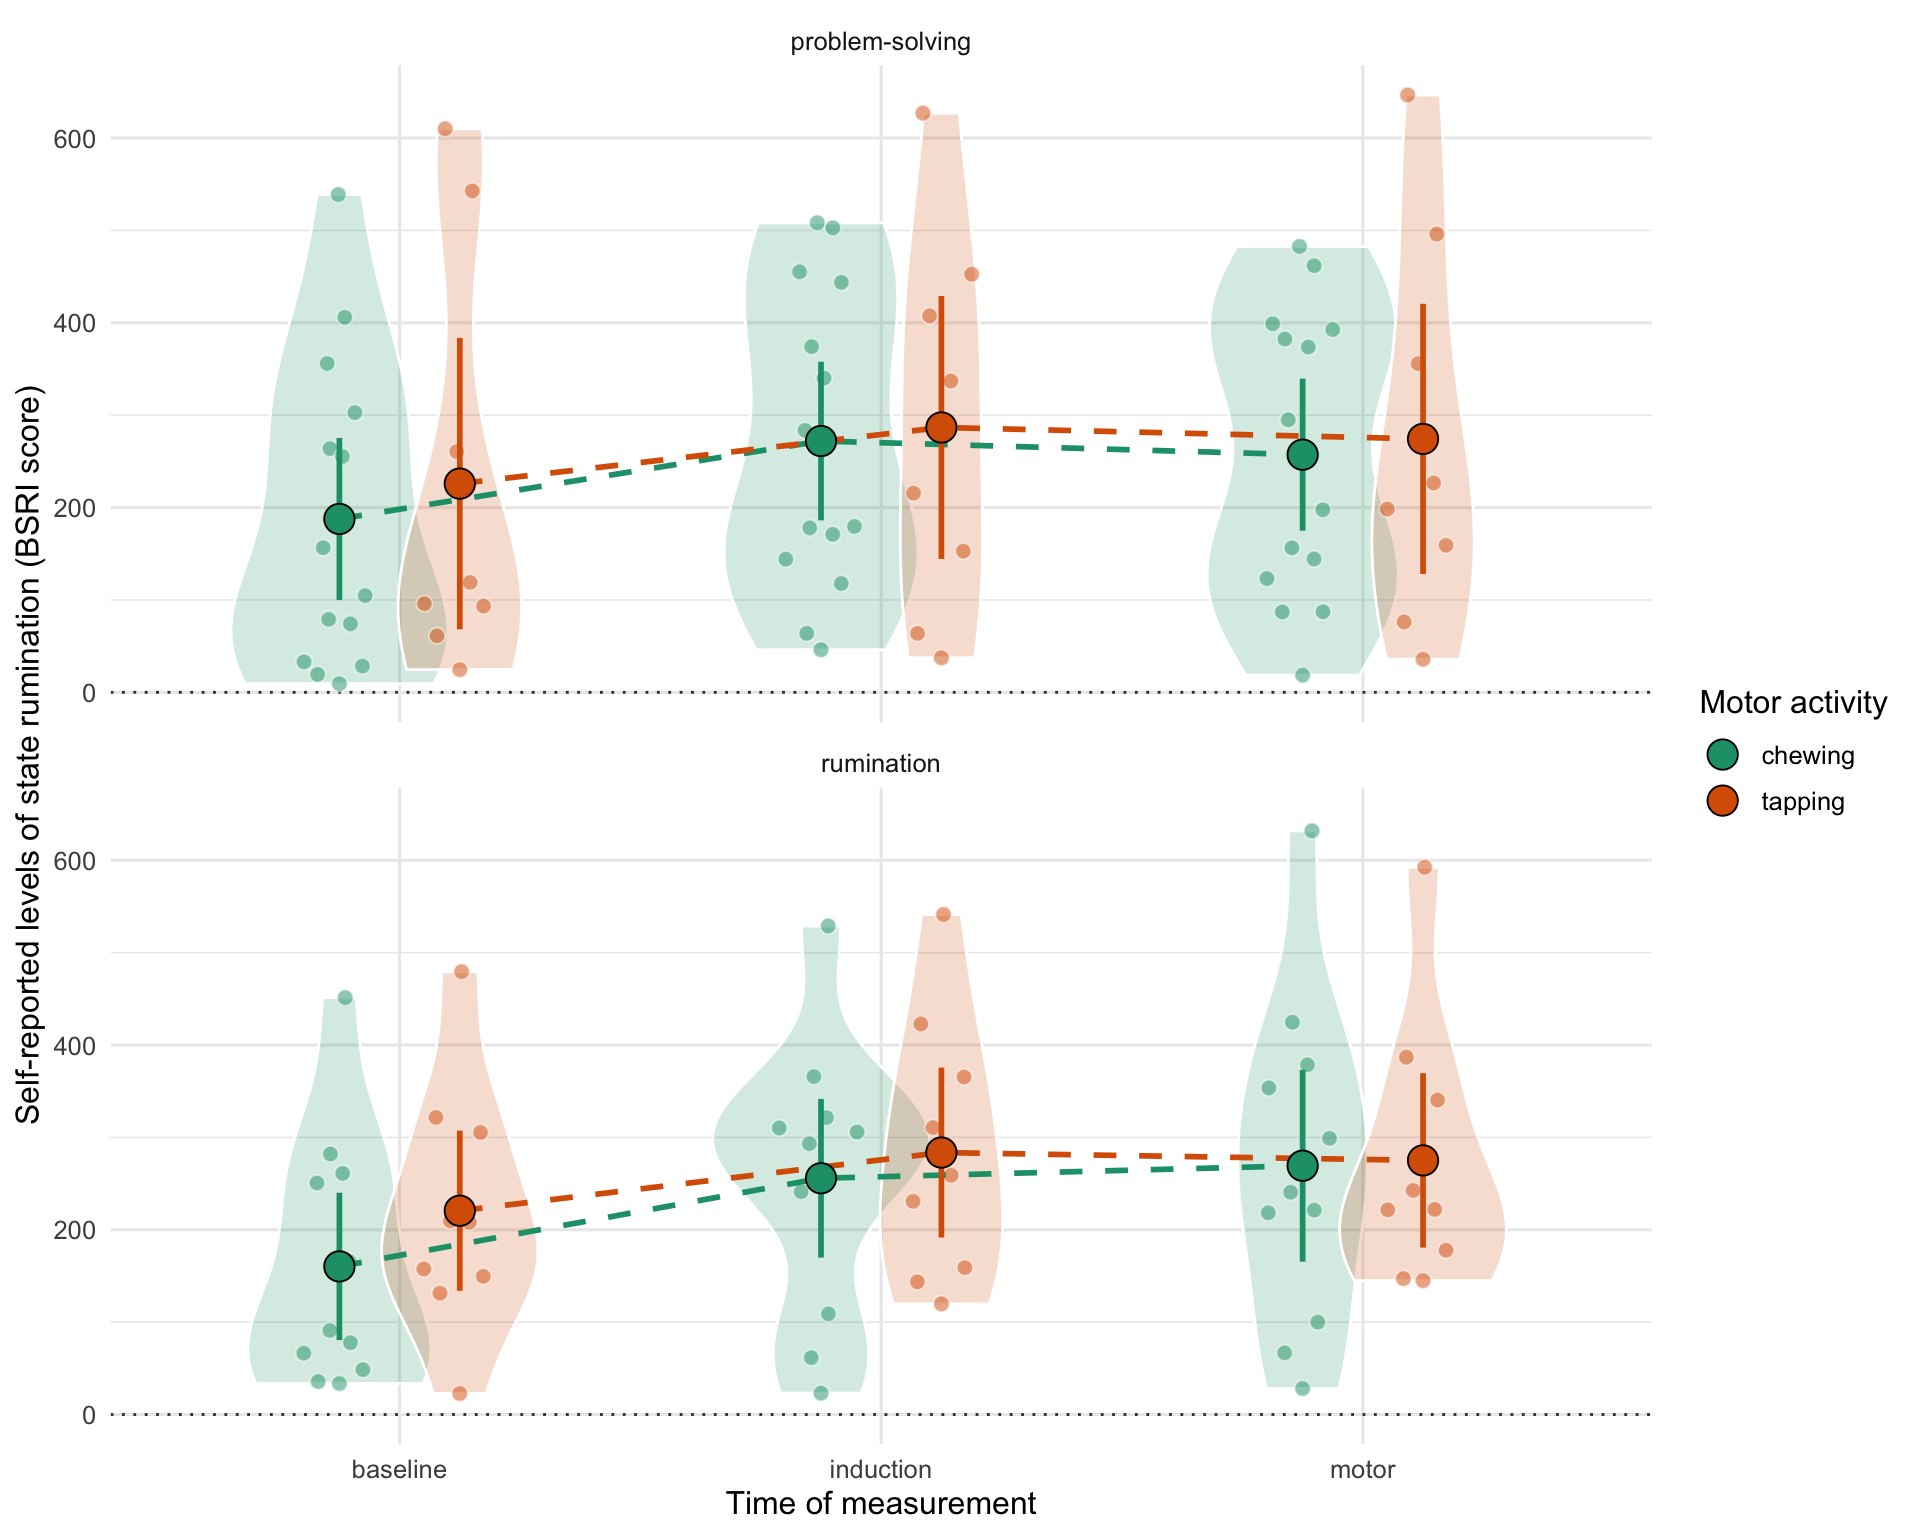
\includegraphics{02-chap2_files/figure-latex/unnamed-chunk-2-1} 

}

\caption{Simulated EMG signal.}\label{fig:unnamed-chunk-2}
\end{figure}

\ldots{}we rectify the EMG signal by taking its absolute value and
substracting the mean in order to correct for any offset (bias) present
in the raw data. It is interesting to note that the effects of
rectification on the EMG signal is similar to the rectification of AM
radio waves whose purpose is to enhance the low frequency components,
wich encode the voice signals. Concerning EMG, the ``voice'' of the
signal corresponds to the encoded force \citep{Borg2007}.

\begin{Shaded}
\begin{Highlighting}[]
\OperatorTok{>}\StringTok{ }\NormalTok{emg <-}\StringTok{ }\KeywordTok{abs}\NormalTok{(emg }\OperatorTok{-}\StringTok{ }\KeywordTok{mean}\NormalTok{(emg) )}
\OperatorTok{>}\StringTok{ }\KeywordTok{ts.plot}\NormalTok{(emg, }\DataTypeTok{xlab =} \StringTok{"Time (ms)"}\NormalTok{, }\DataTypeTok{ylab =} \StringTok{"simEMG"}\NormalTok{, }\DataTypeTok{col =} \StringTok{"steelblue"}\NormalTok{)}
\end{Highlighting}
\end{Shaded}

\begin{figure}[h!]

{\centering 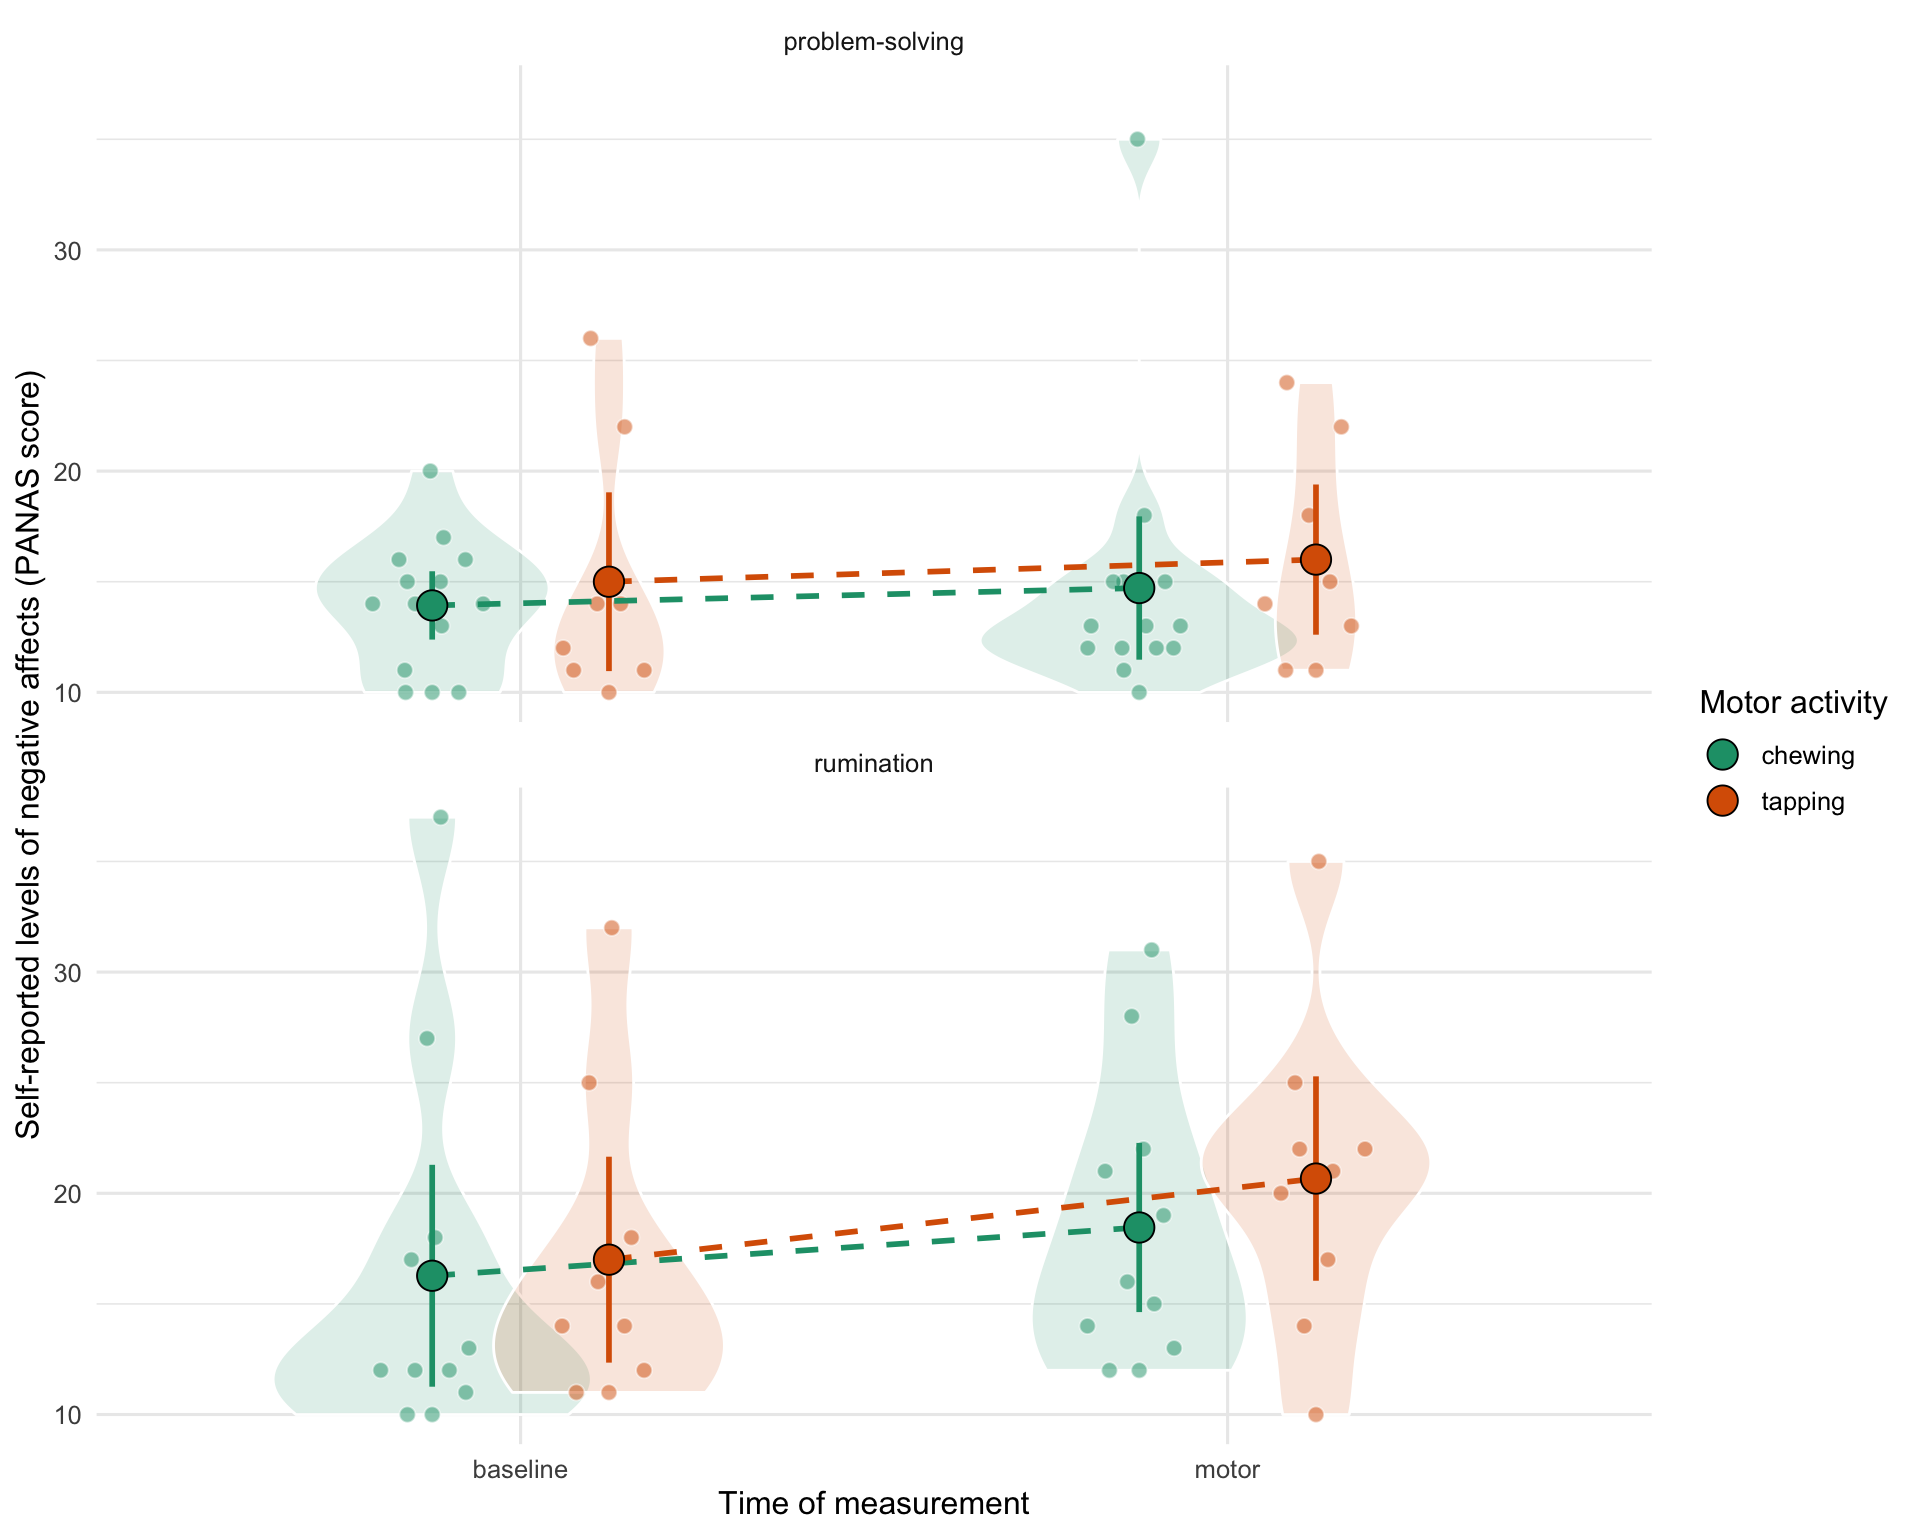
\includegraphics{02-chap2_files/figure-latex/unnamed-chunk-3-1} 

}

\caption{Rectified EMG signal.}\label{fig:unnamed-chunk-3}
\end{figure}

\ldots{}

There are two main measures thant can be used to represent the magnitude
of muscle activity. These two measures can be directly computed from the
filtered EMG signal. The first one is the \textbf{average rectified
value} (ARV):

\[ARV = \frac{1}{T} \sum_{t=1}^{T} | EMG(t_{i}) |\]

which is computed over a specific interval \((0,T)\) and where
\(|EMG(_{i})|\) is the absolute value of a datum of EMG in the data
window. The unit of measurement is \(mV\) or \(\mu V\), and the ARV
calculation is generally similar to the numerical formula for
integration \citep{Kamen2010}.

The second one is the \textbf{root-mean-square} (RMS) amplitude:

\[RMS = \sqrt \frac{1}{T} \sum_{t=1}^{T} | EMG^{2}(t_{i}) |\]

where \(|EMG^{2}(_{i})|\) is the squared value of each EMG datum and has
both physical and physiological meanings\ldots{}

\part{Experimental part}\label{part-experimental-part}

Blah blah blah\ldots{} explain why two parts\ldots{}

\chapter{Orofacial electromyographic correlates of induced verbal
rumination}\label{orofacial-electromyographic-correlates-of-induced-verbal-rumination}

Biological Psychology paper\ldots{}

\chapter{Dissociating facial electromyographic correlates of visual and
verbal induced
rumination}\label{dissociating-facial-electromyographic-correlates-of-visual-and-verbal-induced-rumination}

Second EMG study with Sonja\ldots{}

\chapter{Zygoto experiment}\label{zygoto-experiment}

\ldots{}

\chapter{Articulatory suppression effects on induced
rumination}\label{articulatory-suppression-effects-on-induced-rumination}

\ldots{}

\chapter{TMS study}\label{tms-study}

\ldots{}

\part{General discussion and
conclusions}\label{part-general-discussion-and-conclusions}

\chapter{General discussion}\label{general-discussion}

\ldots{}

\chapter{Conclusions}\label{conclusions}

\ldots{}

\chapter*{References}\label{references}
\addcontentsline{toc}{chapter}{References}

\markboth{References}{References}

\singlespacing
\sloppy

\noindent

\setlength{\parindent}{-0.20in} \setlength{\leftskip}{0.20in}
\setlength{\parskip}{8pt}

\bibliography{bib/book.bib,bib/packages.bib}


\end{document}
